\section{Model Fragmentation}
\label{sec:fragmentation}

\subsection{Fragmentation in General}
All models considered in this paper can be characterized as directed labeled graphs with a fix spanning-tree called \emph{containment hierarchy}. In EMF based models, the containment hierarchy consists of \emph{containment references}; other graph edges are \emph{cross-references}. 

Model fragmentation breaks (i.e. \emph{fragments}) a model along its containment hierarchy. All \emph{fragments} are disjoint; no object is part of two fragments. Fragmentation is also always complete, i.e. each object is part of one fragment. The set of fragments of a model is called \emph{fragmentation}. References between fragments are called inter-fragment and references within a fragment are called intra-fragment references.~\footnote{Based on these characteristics, fragments can be compared to EMF's resources (especially with containment proxies); refer to section~\ref{sec:implemention}, where we use resources to realize fragmentation.} 

\begin{figure}[ht]
\centering
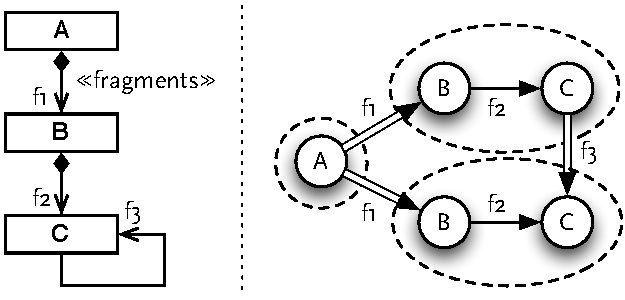
\includegraphics[width=0.65\linewidth]{figures/fragmentationExplained}
\caption{Example meta-model (left) and model (right). In the model: dashed ellipses denote fragments, double lines inter- and normal lines intra-fragment references. The references of feature \emph{f1} determine the fragments, the reference of \emph{f3} is a inter-fragment cross-reference by accident.}
\label{fig:metamodelFragmentation}
\end{figure}  

\subsection{Fragmentation Strategies}

Originally a model is not fragmented; once it was fragmented, the fragmentation needs to be maintained when the model is modified. Further, we have to assume that fragmentation has an influence on performance (refer to sections~\ref{sec:gains} and~\ref{sec:evaluation}). We denote a set of algorithms that allows to create and maintain a fragmentation as \emph{fragmentation strategy}.

There are two trivial strategies: \emph{no fragmentation} and \emph{total fragmentation}. No fragmentation means the whole model constitutes of one fragment, such as in EMF (without resources). Total fragmentation means each object constitutes its own fragment. There are as many fragments as objects in the model. This strategy is implemented by existing persistence frameworks like CDO.

\subsection{Meta-Model based Fragmentation}

In this paper, we propose and use \emph{meta-model based fragmentation} as fragmentation strategy. A meta-model defines possible models by means of classes and their attribute as well as reference features. Whereby, the meta-model determines which reference features produce containment and which produce cross-references. The meta-modeler already uses containment reference features to aggregate related objects.

In meta-model based fragmentation, we ask the meta-modeler to additionally mark those containment reference features that should produce inter-fragment containment references. 
This way, the meta-model determines where the containment hierarchy is broken into fragments, and it becomes easy to create and maintain fragmentations automatically and transparently (ref. to section~\ref{sec:implemention}). Only containment reference features determine fragmentation, cross-references can become inter-fragment references by accident. See Fig.~\ref{fig:metamodelFragmentation} for an example.

%Only containment features can be designated as inter-fragment reference features and all instances of such a reference feature will be inter-fragment references (like \texttt{a}-references in Fig.~\ref{fig:metamodel_fragmentation_pattern_tree}). Other references (i.e. cross references) can become inter-fragment references \emph{by accident} (like \texttt{c}-references in Fig.~\ref{fig:metamodel_fragmentation_pattern_graph}).


%\subsubsection{Theory}
%Access patterns for a model are strongly influenced by its metamodel.
%Metamodels are tiny in comparison to their large instances. 
%If you imagine looking from above onto a large model, the metamodel types of its objects form patterns. How we access a model is also influenced by its metamodel, since all algorithms doing something with a model are programmed against its metamodel.
%Hence, optimal fragmentation goes along this patterns.
%Most fragments will have the same structure, and fragments are connected through structural features of only few different types.
%One way to define fragmentation is to mark these fragment crossing structural features. 
%
%Fig.~\ref{fig:metamodel_fragmentation_pattern_tree} shows a simple example metamodel type pattern. The instances (links) of feature \emph{a} cross fragment borders (inter fragment links). All other links are intra-fragment links. The situation is a  little more complicated in Fig.~\ref{fig:metamodel_fragmentation_pattern_graph}. Here the links of feature \emph{c} have both inter- and intra-fragment instances. 
%
%If we want to describe fragmentation by marking features as inter- or intra-fragment features, it would work for the example in Fig.~\ref{fig:metamodel_fragmentation_pattern_tree}, but not for the example in Fig.~\ref{fig:metamodel_fragmentation_pattern_graph}. Obviously, we need further restrictions.
%
%Models (as used in this paper) always have a inherent spanning tree. The spanning tree is formed from links that are instances from containment features. All instances of containment features are part of the spanning tree. If we only allow containment features to be inter-fragment features then the instances of inter-fragment feature will always define a unique fragmentation. \markus{Proof?}
%
%\subsubsection{Implementation}
%This describes an implementation based on EMF. 
%
%\subsection{Automated Fragmentation based on Expected Range Queries}
%\subsection{Automated Fragmentation based on Access Patterns}
%\subsection{Fragmentation of Even Models}
%
%\subsubsection{Analysis}
%
%At the beginning, we will look at \emph{even} models. A model is even, if its inner structure suggest fragmentation into equal pieces. For example, an intuitive way to fragment a OO software model is to put each package into one entry. This is an uneven model, since packages have different sizes. Another example is sensor data, sensor data produced at each point in time or on each node has the same size. If one puts each sensor reading or each node into one entry, the entries will have similar size.
%
%Previously, we were looking the gains achieved with optimal fragmentation. While optimal fragmentation is plausible in manually fragmented models for a single specific loaded model (e.g. accessing single sensor readings in ClickWatch). Optimal fragmentation is unlikely for different loaded models (even impossible for models of different size). 
%
%In general, we can assume that the smaller $ope$ is compared to $load$, the more likely it is that much of each entry is part of the loaded model. In other words, the smaller my entries are, the more likely it is that much or all if a single entry is part of the loaded model. We will model $part$  accordingly.